\documentclass[11pt,french,a4paper]{article}
\usepackage[utf8]{inputenc}
\usepackage[french]{babel}
\usepackage[T1]{fontenc}
\usepackage{fancyhdr}
\usepackage{fancybox}
\usepackage{lastpage}
\usepackage{graphicx}
\usepackage[left=2cm,right=2cm,top=2cm,bottom=2.5cm]{geometry}
\geometry{a4paper}
\setlength{\parindent}{0pt}
\usepackage{listings}
\usepackage{color}
\usepackage[table]{xcolor}
\usepackage{array}
\usepackage{listings}
\usepackage{hyperref}
\usepackage{caption}
\usepackage{lastpage}
\pagestyle{fancy}

\fancyhead[L]{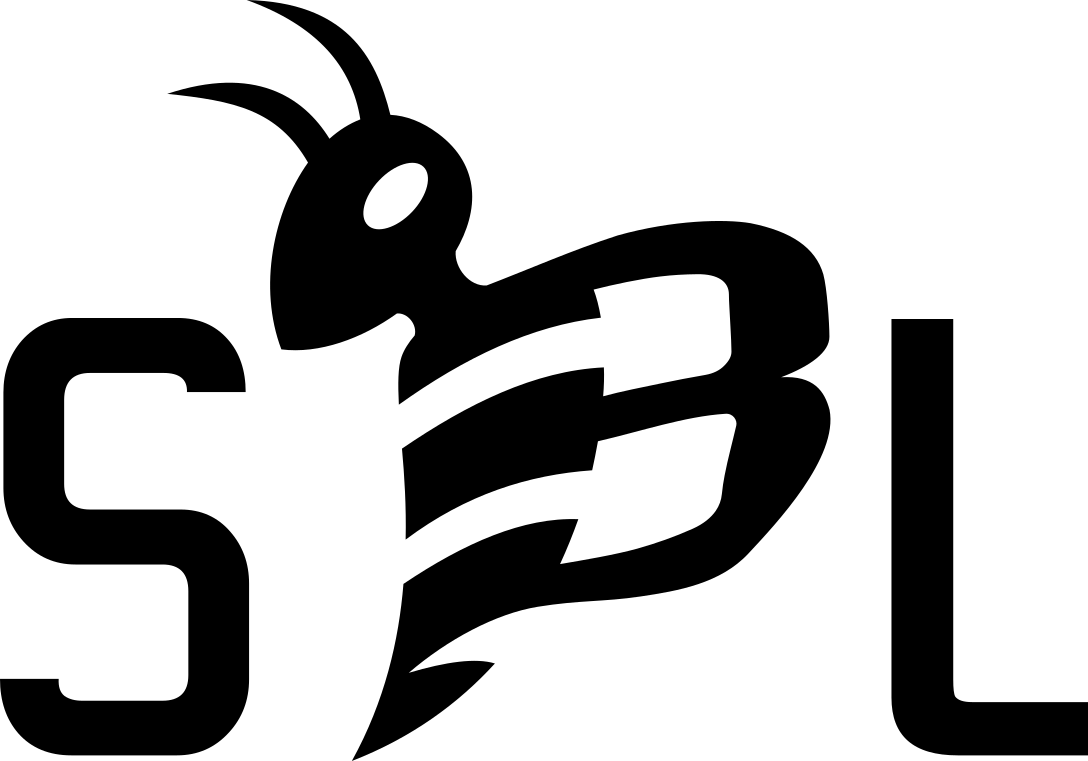
\includegraphics[width=1cm]{../../../logo/SBLlogo.png}}
\fancyhead[C]{Rapport d'activités semaines du 11 et 18 avril 2022 }
\fancyhead[R]{}
\fancyfoot[L]{\small Tom TUELEAU\normalsize}
\fancyfoot[C]{}
\fancyfoot[R]{\thepage/\pageref{LastPage}}


\lstset{
  basicstyle=\fontfamily{lmvtt}\selectfont\small,
  columns=fullflexible,
}

\title{
 \centering
         
\includegraphics[width=4cm]{../../../logo/IUTlogo.png}  \hspace{7cm}
         
\includegraphics[width=4cm]{../../../logo/UMlogo.png}  \hspace{7cm}
    
	\LARGE{Rapport d'activités semaines 25 avril et 18 m<ai 2022 }
	\author{TUELEAU Tom}
}
\author{
	\date{}
}
\begin{document}
\maketitle
	 
\includegraphics[width=4cm]{../../../logo/LIRMMlogo.png}  \hspace{7cm}
         \includegraphics[width=4cm]{../../../logo/IBMMlogo.jpg}  \hspace{7cm}
\newpage
\tableofcontents
\newpage
\section{Introduction}
Ce document a pour objectif de faire un état d'avancement du stage. Celui-ci résumera donc le travail fait lors de la fin du mois d'avril et la premier moitié du mois de mai.
\\Dans un premier temps, je reviendrait sur le montage amplificateur vue lors du dernier rapport et vous montrerait les résultats obtenue.
\\Une seconde partie présentera les programmes crée afin de récolter et traiter les données des capteurs. 
\\Une troisième partie traitera de l'envoie des données entre les différents élément du système.
\\Enfin, je conclurait sur le travail effectuer et les difficultés rencontrer. 

\section{Finalisation du montage}
Lors des précédent rapport, je vous ais exposer mes recherches et résultats quand au dimensionnement d'un montage amplificateur. Dans cette partie nous verrons tout d'abords la finalisation du montage et dans un second temps nous verrons l'installation de cellui-ci dans le rucher.\\
\subsection{Montage}
Lors de cette semain j'ai pu effectuer le prototype final incluant l'amplification du signal, le piézo-électrique, le capteur de température et d'humidité (Si7021) et l'Arduino. Vous pouvez voire un schéma complet Figure \ref{SMG}.
\begin{center}
    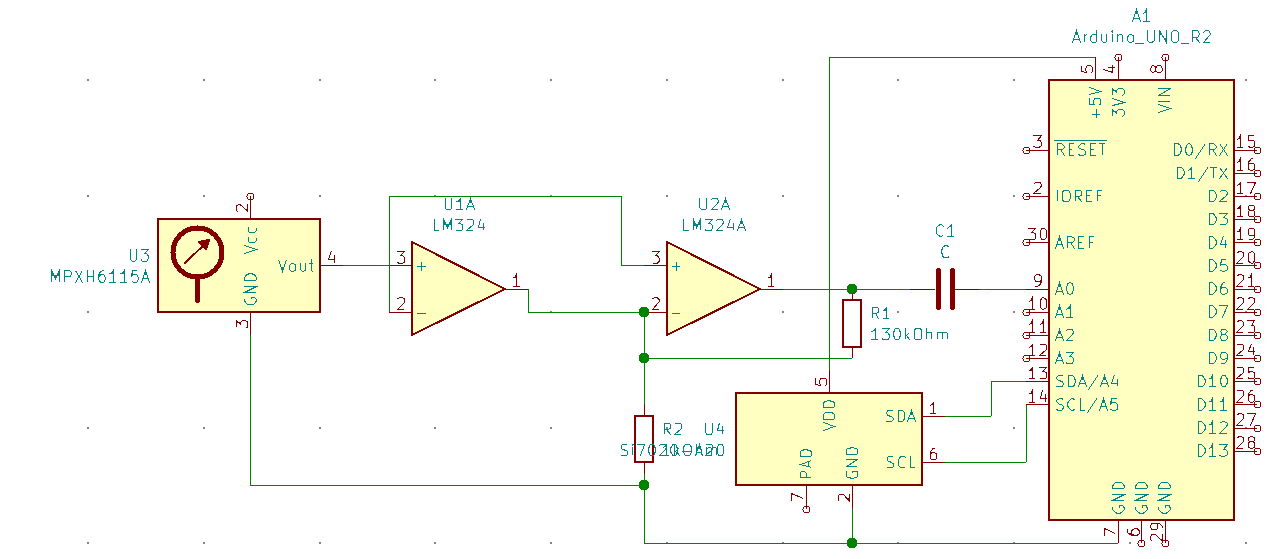
\includegraphics[scale=0.5]{../img/SMG.png}
    \captionof{figure}{Schéma montage final}
    \label{SMG}
\end{center}



\subsection{Installation dans la ruche}
\subsection{Amélioration}
\section{Programmation des capteurs}
\subsection{Capteur de température et humidité}
\subsection{Capteur de vibration}
\subsection{Traitement des données}

\section{Programmation réseaux}
\subsection{Liaisons MQTT}
\subsection{Liaisons UDP}

\newpage
\listoffigures
\end{document}
